\chapter{Conclusions and Further Work}
This chapter summarizes the conclusions that can be drawn from the
results that are presented in this thesis and presents several ideas for
further development of the contributions that have been made.

\section{Further Work}
\label{sec:furtherwork}
This section introduces some relatively new learning algorithms that have
also been developed for operation in continuous multi-dimensional domains and
might also be used to simulate electricity trade.
% Also, two new reinforcement learning problem formulations are defined that
% concern two highly pertinent issues in electric power Engineering.
It also explains is how data from National Grid Ltd.~could be used in practical
simulations of the UK electricity market and some of the posibilities that AC
optimal power flow brings to to electric power market simulation.

\subsection{Alternative Learning Algorithms}
This thesis has concentrated on traditional value function based and two policy
gradient reinforcement learning methods.  However, there have been some
interesting new learning algorithms presented recently and they might also be
examined in the domain of electric power trade.

\citeA{riedmiller05nfq} presented Neuro Fitted Q Iteration (NFQ) algorithms
that attempt to overcome many of the problems experienced when implementing
Q-learning methods with value function approximation using neural networks.
They store all transition experiences and perform off-line updates using
supervised learning techniques such as RProp \cite{riedmiller93}.  The method
has been shown to be robust against parmeterisation and to learn quickly in
standard benchmark tests and in real-world applications \cite{kietzmann09}.

The GQ$(\lambda)$ algorithm by \citeA{maei10} is another extension of the
Q-learning method for operation in continuous spaces.  Convergence guarantees
have been shown and the scaling properties suggest it is suitable for large-scale reinforcement learning
applications.  Software implementations of GQ$(\lambda)$ are reportedly in
development and due to be made available soon.

Four new Natural Actor-Critic algorithms are presented in \citeA{bhatnagar09}.
They all use function approximation techniques, making them suitable for
large-scale applications of reinforcement learning.  Three of the algorithms
are extensions to ENAC \cite{peters:enac}, but are fully incremental: the
gradient computation is never reset while the policy is updated at every
simulation step.  The authors state a need to assess the ultimate utility of
these algorithms through application in real-world problems.

This thesis provides a framework that would allow implementations of these
interesting new algorithms to be assessed and used to examine aspects of
electricity markets.

% \subsection{Learning to Optimise Power Flow}
% Two important problems in electric power Engineering, to which to the
% application of advanced reinforcement learning algorithms would be of value,
% are:
% \begin{itemize}
%   \item System optimisation, close to real-time, such that sufficient reserve
%   is allocated to ensure acceptable system security while costs are minimised
%   according to the outcome of the electricity markets, and
%   \item Capital investment planning, both by system operators needing to expand
%   transmission capacity and energy companies wanting to develop new generating
%   plant.
% \end{itemize}
%
%
% As explained in Section \ref{sec:opf}, the objective of the classical optimal
% power flow problem is to find generator set-points that allow all system and
% plant constraints to be satisfied while the total system cost is minimised.
% Interior point methods are possibly the most robust technique for finding
% solutions, but the problem may also be formulated as a continuous
% reinforcement learning task that could be learned by a system operator agent.
% To illustrate the concept, this section presents a preliminary formulation of
% such a task and demonstrates how a system operator agent can use policy
% gradient methods to learn to optimise power flow.
%
% \subsubsection{System Operator Task and Environment}
% The state of the system operator agent's environment is defined simply as a
% demand forecast.  That is, the environment returns a vector of active power
% demand at all system buses.  The initial demand is assumed to be peak and is
% used to normalise the values of the sensor vector to be between $-1$ and $+1$
% before input the the mutil-layer perceptron used for policy function
% approximation.  Simulations are divided into episodes (days) over which the
% demand at each bus follows the profile shown in Figure X.
%
% The agent's action and the output of the policy function approximator is a
% vector of the active power set-points of all generators, excluding the
% generator at the system slack bus.  The set-points are bound by the generator's minimum
% and maximum rated capacity. These bounds are used to denormalise the output
% values from the final Sigmoid layer (that are between $-1$ and $+1$) to give
% valid set-point values.
%
% The new generator set-points are used to form an AC power flow problem that is
% solved using Newton's method \cite{tinney:67}.  The power flow solution
% determines the complex voltage at each bus, the branch power flows and losses,
% the reactive power output of the generators and the active power output of the
% slack bus generator.
%
% The reward is defined as the negative of the sum of all generator costs.  The
% negative of the costs must used since the learning methods attempt to maximise
% reward and the objective is to minimise cost.  The power flow solution does not
% satisfy system constraints, such as voltage limits or generators reactive power
% limits and penalty costs must be applied to the reward so the agent learns to
% obey them.
%
% \subsubsection{Slack Bus Generator Control}
% This initial proof of concept attempts only to enforce the set-point limit on
% the slack bus generator.  The reward is updated according to
% \begin{equation}
% r =
% \begin{cases}
% r + \phi (P_{slack} - P_{max}), & \text{$P_{slack} > P_{max}$} \\
% r, & \text{otherwise}
% \end{cases}
% \end{equation}
% The six bus network model described in Chapter \ref{ch:nashanalysis} is used
% with the coefficients of the generator's quadratic cost functions given in Table X.  Learning is conducted in batch
% mode, with 7 episodes conducted before the parameters of the policy are
% updated.  The system operator agent uses the ENAC learning method with RProp
% gradient descent and an initial value of $\sigma = 50$, which is reduced after
% each simulated week according to $\sigma_{i+1} = 0.5\sigma_i - 2$.
%
% Figure X shows the average output of each generator over 52 simulated weeks of
% control. Plotted in Figure Y is the average total system cost for each week along with
% theoretically optimal values as calcualted by DC and AC optimal power flow
% solvers.  The results show that, with suitable initial experimentation, the
% agent learns to dispatch the generators in the most economically efficient
% manner while controlling the slack bus generators to valid output levels.  The
% average total system cost converges to slightly less that of the optimal
% solution due to the disregard for other constraints, particularly the
% branch flow constraint between buses 2 and 4 which is binding at times of peak
% load.
%
% \subsection{Learning to Plan Investment}

\subsection{UK Transmission System}
Some of the more ambitious agent-based electricity market simulations have used
stylised models of national transmission systems
\cite{cincotti:09,weidlich:06}.  This work has often been motivated by recent
or expected changes to the arrangements in the associated regions.

% The drop in
% oil prices around the time of the global economic crash in 2008 was not
% reflected quickly in energy prices and this amplified concerns over liquiduty
% levels in the UK electricity markets.  Ofgem found competition to be
% sufficient[ref], but the concerns persists and the market arrangements have
% been re-examined under Project Discovery[ref].

Several of the the UK's largest power stations are due to be decommissioned
around 2015 in accordance with EU Large Combustion Plant Directive.  The
ability of the market to sufficiently incentivise new investment in generation
that will cover the resulting shortfall is in question.  The concern extends
to the need for long-term investment in new nuclear power plant that is deemed
neccessary for the UK to meet the legally binding obligations, made in the
Climate Change Bill, to cut greenhouse gas emissions by 80\% by 2050, compared
to 1990 levels.

Examination of the situation could be enhanced by the advanced participant
behavioural models and the accurate electric power system simulations
presented in this thesis.  Figure \ref{fig:ngt_grid} illustrates a model of
the UK transmission system that has been derived from data provided in
\citeA{ngtsys2010}.  This model has been converted into a PSS/E version 30 raw
file and is distributed with the code developed for this thesis (See Appendix
\ref{sec:pylon}).
%Generator set-points were determined using the state estimator from Pylon
% [Crow].  The power flow results are shown in Figure X and correlate
% accurately with those in [SYS], having a mean variance of X.XX.
% Cost data for each of the aggregated generating units has
% been estimated from public sources and stored in the PSS/E version 30 optimal
% power flow data file in Appendix \ref{sec:nget_opf}.  Execution times for
% solving this case using DC, AC and unit de-commitment optimal power flow are
% shown in Table X.

\ifthenelse{\boolean{includefigures}}{
	\begin{figure}
	  \centering
	  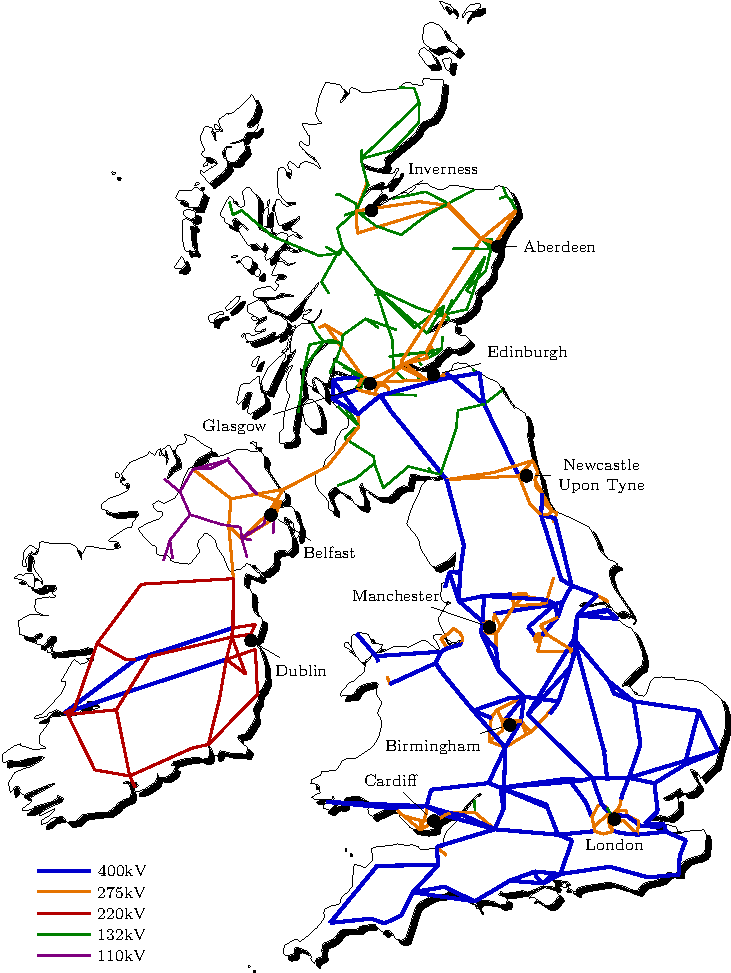
\includegraphics{figures/ngt_grid}
	  \caption{UK transmission system.}
	  \label{fig:ngt_grid}
	\end{figure}
}{}

It is currently too computationally expensive for this model to be solved
repeatedly in an agent-based simulation.  However, optimisation efforts might
allow for it to be used to examine issues pertinent to the UK energy industry.

% However, significant improvements in
% speed should be possible through more efficient construction of the Hessian
% matrices in the AC optimal power flow solver.  Agent-based simulation lends
% itself to parallelisation and the artificial neural networks could be
% processed in multiple threads on multi-core processors or on distributed
% memory architectures.

\subsection{AC Optimal Power Flow}
To the best of the author's knowledge this is the first application of AC
optimal power flow in agent-based electricity market simulation.  AC optimal
power flow formualtions are more difficult to implement and the problems are
more computationally expensive than than their linearised DC counterparts.  The
additional time and effort does not always bring sufficient value to
electricity market simulations.  However, the option to use an AC formulation
offers some interesting possibilities for further work.

The inclusion of reactive power costs in the objective function of an AC
optimal power flow problem means that parallel auctions for voltage support
could be added to simulations.  This could be open to agents associated with
reactive compensation equipment such as that commonly needed for wind farm
developments.  Reactive power markets have traditionally been largely
academic, but as the UK makes greater use of wind power the topic could
become of increasing interest.

Bus voltages are not all assumed to be 1~per-unit in AC optimal power flow
problems, but are part of the vector of optimisation variables.  Adjusting
phase shift angles, $\theta_{ph}$, offers a degree of control over the
direction of power flows.  The control the transformer tap ratios, $\tau$, and
the shift angles by learning agents could be of interest in the evaluation of
congestion management techniques.

\subsection{Multi-Market Simulation}
% Policy gradient method's superior use of sensory data and their ability to
% operate in large action domains opens opportunities for more detailed study of
% inter-market relationships.
The global economy is a holistic system of
systems and the anaylsis of markets independently must be of limited value.
Recent agent-based electricity market simulations studies have investigated the
interaction between electricity, gas and emission allowances markets
\cite{krause:gas,wang:09}.
% Non-linear models [ref] have been published for gas flows in pipelines such as
% those of the UK gas network.
The information on the UK gas network provided in \citeA{ngtsys2010} is
relatively limited to that of the electricity transmission system, but
suitable models could be used in conjunction to study the the relationsships
between gas and electricity markets.  As in \citeA{krause:gas}, actions in the
gas market would constrain the generators options to sell power in subsequent
electricity auctions.  Add to this the option to trade in carbon markets and
the agent's state and action spaces would quickly become very large and
suitable learning methods would be required.

% \subsection{Common Information Model}
% Many tools exist for steady-state analysis of balanced three-phase AC networks
% and most are centred around bespoke models that describe the power system
% data.  Several attempts have been made in the past to standardise the format
% in which power system data is stored [CDF, UKGDS, ODF] and latest and most
% popular is the Common Information Model.
%
% The Common Information Model (CIM) is an abstract ontological model that
% describes the elements of national electric power systems and the associations
% between them.  CIM is an evolving international standard approved by the
% International Electrotechnical Commission (IEC).
%
% Unlike many tool specific models the CIM does not simplify the power system
% into a graph of buses connected by branches.  Instead it describes each of the
% components in the system and the electrical connectivity between them.
% Conventional numerical techniques for steady-state analysis of AC power
% systems require a simplified bus-branch model such that when the voltage angle
% and magnitude at each bus is determined the power flows on each branch may be
% calculated.

% market power, constraint management
%\section{Decentralised Trade}
% distribution level, renewables
%\section{Standarisation}
% CIM for markets
%\section{Blackbox optimisation}
% periodic

%\subsection{Summary}

\section{Summary Conclusions}
\label{ch:conclusion}

% restate contributions